\documentclass{standalone}
\usepackage{tikz}
\usepackage{ctex,siunitx}
\setCJKmainfont{Noto Serif CJK SC}
\usepackage{tkz-euclide}
\usepackage{amsmath}
\usetikzlibrary{patterns, calc}
\usetikzlibrary {decorations.pathmorphing, decorations.pathreplacing, decorations.shapes,}
\begin{document}
\small
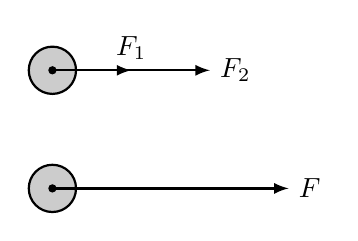
\begin{tikzpicture}[>=latex, thick,scale=1]
  % \useasboundingbox(-1,-0.75)rectangle(3.7,1.4);
  \draw [fill=black!20](0,1.5) circle[radius=.3];
  \fill (0,1.5) circle[radius=1.5pt];
  \draw [->](0,1.5)--(1,1.5) node [above] {$F_1$};
  \draw [->](0,1.5)--(2,1.5) node [right] {$F_2$};
  \draw [fill=black!20](0,0) circle[radius=.3];
  \fill (0,0) circle[radius=1.5pt];
  \draw [->](0,0)--(3,0) node [right] {$F$};
  \end{tikzpicture}
\end{document}